Dieses Experiment testet, wie anfällig die Agenten für Verklemmungen sind.

\textbf{Aufbau des Experiments}
\begin{figure}[H]
    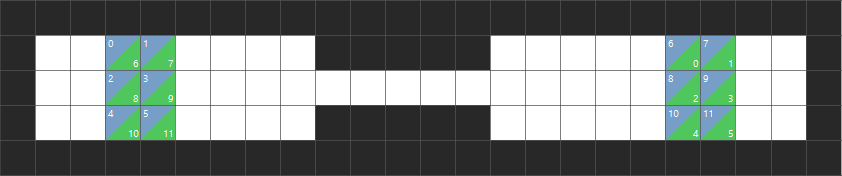
\includegraphics[width=\textwidth]{images/tunnel_2_groups.png}
    \centering
    \caption{Ausgangssituation für das Durchqueren eines Tunnels von zwei Gruppen, bestehend aus jeweils sechs Agenten}
    \label{fig:tunnel}
\end{figure}
In diesem Experiment durchqueren zwei Gruppen aus jeweils sechs Agenten eine Engstelle, die fünf Felder lang und ein Feld breit ist. Jeder Agent muss die Engstelle passieren um sein Ziel zu erreichen.

\textbf{Erwartete Beobachtungen}\newline
Im ersten Schritt nähern sich beide Gruppen der Engstelle. Während eine Gruppe anfängt die Engstelle zu durchqueren, fahren die Agenten der anderen Gruppe Ausweichpositionen an und verlängern damit die Engstelle. Im Laufe des Experiments wechseln die Gruppen ihre Rollen häufiger.